\documentclass[10pt,a4paper]{article}
\usepackage[utf8]{inputenc}
\usepackage[spanish]{babel}
\usepackage{amsmath}
\usepackage{amsfonts}
\usepackage{amssymb}
\usepackage{enumitem}
\usepackage{longtable}
\usepackage{ltablex,booktabs}
\usepackage{hyperref} 
\usepackage{graphicx}
\usepackage[table]{xcolor}
\hypersetup{pdftex,colorlinks=true,allcolors=blue}
\hypersetup{
    pdftitle={},
    pdfauthor={Pablo Riutort Grande},
    pdfsubject={},
    bookmarksnumbered=true,     
    bookmarksopen=true,         
    bookmarksopenlevel=1,       
    colorlinks=true,            
    pdfstartview=Fit,           
    pdfpagemode=UseOutlines,    % this is the option you were lookin for
    pdfpagelayout=TwoPageRight
}
\usepackage{geometry}
\usepackage{listings}
\usepackage{xcolor}
\usepackage{hypcap}
\definecolor{codegreen}{rgb}{0,0.6,0}
\definecolor{codegray}{rgb}{0.5,0.5,0.5}
\definecolor{codepurple}{rgb}{0.58,0,0.82}
\definecolor{backcolour}{rgb}{0.95,0.95,0.92}
\lstdefinestyle{mystyle}{
    backgroundcolor=\color{backcolour},   
    commentstyle=\color{codegreen},
    keywordstyle=\color{magenta},
    numberstyle=\tiny\color{codegray},
    stringstyle=\color{codepurple},
    basicstyle=\ttfamily\footnotesize,
    breakatwhitespace=false,         
    breaklines=true,                 
    captionpos=b,                    
    keepspaces=true,                 
    numbers=left,                    
    numbersep=5pt,                  
    showspaces=false,                
    showstringspaces=false,
    showtabs=false,                  
    tabsize=2
}

\lstset{style=mystyle}
\usepackage{xparse}
\NewDocumentCommand{\codeword}{v}{%
\texttt{{#1}}
}
\author{Pablo Riutort Grande}
\title{
	Seguridad en Bases de Datos\\
	\vspace{0.5cm}
	PEC 1\\
	\vspace{1cm}
	\textbf{Seguridad y pentesting de servidores de datos}
	\vspace{1cm}\\UOC - MISTIC
}
\begin{document}
\maketitle
\pagebreak

\section{}
\subsection{}
Una combinación roles para el escenario presentado podría ser el siguiente:
\begin{itemize}
\item \textbf{DBA (Administrador de Base de Datos)}: Este rol permite definir el schema de la base de datos así como sus usuarios y los permisos de estos. También es el responsable de velar por la seguridad de la base de datos aplicando el plan de seguridad y backups y de reparar los posibles fallos debidos al hardware o al software.
\item \textbf{Administrador de Sistemas}: Este rol es muy similar al anterior exceptuando la definición del schema de la base de datos. También vela por la seguridad de la base de datos y de sus procesos así como los backups y el acceso y disponibilidad a la BD por parte de los usuarios.
\item \textbf{Miembro del departamento de contabilidad}: Este es un usuario normal con permisos restringidos a las tablas que gestionan y relacionan los usuarios con sus sueldos.
\end{itemize}

Los usuarios que podrían adquirir uno o varios de esos roles son los siguientes:
\begin{itemize}
\item \textbf{Usuario del departamento de contabilidad}: Este usuario tiene acceso y permisos de consulta y modificación sobre las tablas relacionadas con la contabilidad de la empresa y sus usuarios.
\item \textbf{CSO}: El CSO es el Responsable de la Seguridad Corporativa. Su función principal es garantizar la seguridad física y la tecnológica.
\item \textbf{Responsable de seguridad}: Se encarga de que el tratamiento de datos personales se realicen conforme al RGPD.
\item \textbf{Personal de seguridad}: Sería la persona que velaría de la seguridad física, en este caso de los equipos, las cintas y su adecuado acceso y transporte.
\end{itemize}

\subsection{}
El plan director de seguridad (PDS) elaborado por el CSO y el Responsable de seguridad deberá ser seguido por todos los usuarios. Algunas de las medidas que puede definir son:
\begin{itemize}
\item Control de acceso físico a las instalaciones: Tarjetas de identificación que deberán llevarse colgadas en todo momento dentro del recinto de trabajo.
\item Control de acceso a los ordenadores: Los equipos están protegidos por usuario y contraseña.
\item Control de acceso a los sistemas de la empresa: Los accesos a servidores, bases de datos, intranets, etc. deberán ser gestionados mediante software adicional de control de acceso como una doble autenticación mediante una app, SSH, LDAP, etc.
\item Control de acceso a la red: A la red se accede mediante la VPN de la empresa y el acceso a esta está gestionado por el equipo de seguridad o el deperatamento de IT. Podría recomendarse el uso de certificados digitales y SSL.
\item Cifrado de disco: Los ordenadores deberán tener el disco cifrado.
\item Control de dispositivos: En caso de traer un dispositivo o equipo externo deberá ser avalado por el departamento de IT y deberá cumplir con las especificaciones que se establezcan.
\item Control de acceso a la base de datos: El DBS podría limitar el acceso a únicamente a través de equipos especiales o servidores jump que estén en una DMZ protegida por firewalls.
\item Realización periódica de backups de los equipos personales y por parte del DBS o del sysadmin backups de las bases de datos.
\end{itemize}

\subsection{}
\subsubsection{}
El nuevo planteamiento supone un cambio significativo en la gestión de las bases de datos de la compañía ACME.\\

El rol de DBA pasa a ser responsabilidad de la compañía de Cloud Computing y desaparece, al menos para esta competencia, de la empresa ACME. El rol de administrador de sistema se mantiene pero este deberá adaptar las necesidades de acceso y seguridad hacia la plataforma de Cloud Computing ya que esta es la que ahora se encarga de la seguridad y acceso de los datos per se, deberá asegurar las conexiones y los posibles accesos a base de datos de manera segura entre ACME y Cloud Computing de la misma forma que lo hacía antes. Dependerá de él entender y evaluar los riesgos de la arquitectura de las dos empresas en este aspecto y velar porque la conexión sea lo más accesible y segura posible.\\
El rol de personal de contabilidad y otros usuarios de la base de datos tendrán las mismas responsabilidades sobre los datos pero deberán adaptarse a la nueva herramienta y quizá modificar algún flujo de trabajo; quizá deban autenticarse de otra forma o conectarse a otros servidores o servicios que permitan la conexión segura entre su ordenador y el cloud.\\
En cuanto a seguridad física, de transporte de las cintas y de acceso a los servidores desaparece y se libera al personal de seguridad de esta responsabilidad.\\Finalmente, el plan de seguridad y tratamiento de los datos deberá actualizarse y coordinarse entre ambas compañías ya que muchas tareas de seguridad de los datos se han visto delegadas pero su uso responsable y acorde con las leyes vigentes sigue siendo responsabilidad de la empresa ACME.

\subsubsection{}
Parte de la seguridad queda externalizada al servicio de Cloud Computing, por tanto, ahora existe esa oportunidad de atacar directamente al servicio de Cloud Computing que es la delegada de la gestión de las bases de de datos de ACME y de quizá otras compañías.\\
También surge la problemática de que el factor humano se multiplica por 2, es decir, hay 2 empresas implicadas en el tratamiento seguro de los datos y por tanto el riesgo se ve incrementado en este aspecto.\\
Surge la oportunidad de atacar una nueva conexión entre ACME y el servicio de Cloud Computing. Anteriormente la conexión a la base de datos estaba gestionada por una sola compañía, ahora hay 2 compañías implicadas y probablemente la de Cloud Computing tenga una arquitectura de seguridad para conexiones externas estandarizada y fácil de conocer y, por ende, de explotar; ahí reside el nuevo riesgo.\\
Finalmente, surge también el riesgo por parte de ACME que surgen a raíz de una posible plataforma de conexión que haya para acceder a la base de datos. Dicha plataforma puede ser un nuevo foco de vulnerabilidades y además vendrá sumado al riesgo que supone para los empleados adaptarse al nuevo uso de manera segura.

\subsubsection{}
ACME deberá implantar un nuevo plan de seguridad que recoja y aglutine la herramienta que ofrezca la empresa de Cloud Computing para acceder a la base de datos. Esto incluye sesiones formativas a los usuarios finales para interactuar de manera segura y eficiente y diseñar e implementar una nueva arquitectura de conexión segura y compatible con ACME por parte del departamento de IT o el administrador de sistemas.\\
Medidas que deberá exigir ACME son las mismas que debía autoexigirse cuando los datos eran responsabilidad suya, que los datos sean accesibles y que se cumpla la normativa vigente en cuanto a su uso y tratamiento. También deberá exigir a la empresa de Cloud Computing que se tenga una información constante sobre noticias de interés que puedan repercutir en ACME tales como nuevas normativas, vulnerabilidades que se descubran y, por supuesto, que se informe en caso de brecha o algún otro evento de importancia que afecte directamente a los datos.

\subsubsection{}
Podría plantearse no externalizarse este servicio cuando los datos sean especialmente sensibles o se vean adscritos a sanciones muy graves en caso de fuga. También si los datos son muy valiosos o las necesidades de la empresa respecto a ellos no se adapten completamente a lo que ofrezca ninguna plataforma de Cloud Computing.\\
Finalmente, también podría no plantearse esta externalización si el coste de la misma, bien económico o de recursos, no valga la pena a mantener el esquema actual.

\subsection{}

En el cluster se han creado 3 usuarios cada uno con un rol diferente.
\begin{figure}[h!]
  \centering
  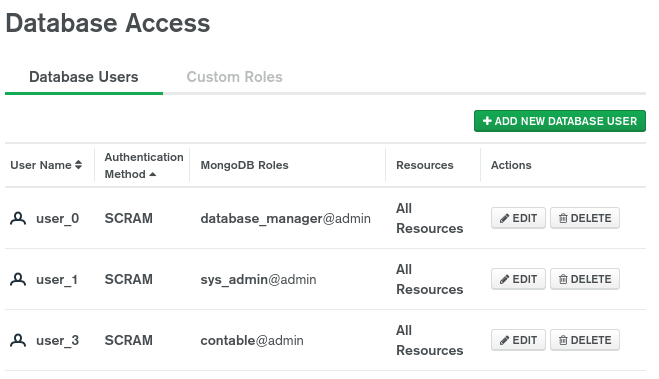
\includegraphics[scale=0.5]{cluster.png}\\
  \caption{Usuarios del cluster}
  \label{fig:cluster_users}
\end{figure}

El rol de DBA tiene todos los permisos posibles sobre la base de datos.
\begin{figure}[h!]
  \centering
  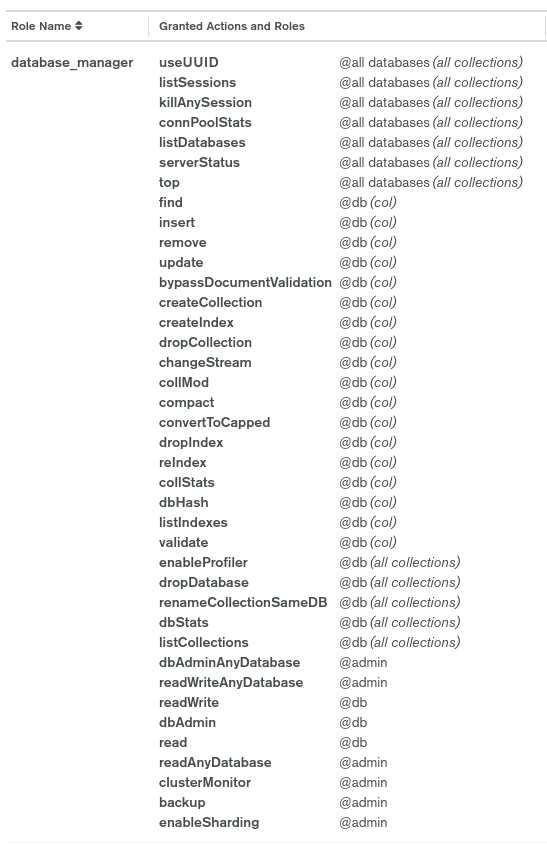
\includegraphics[scale=0.5]{dba.png}\\
  \caption{Rol de DBA}
  \label{fig:dba}
\end{figure}


El rol de sys\_admin tiene todos los permisos posibles sobre la base de datos excepto los que modifican el schema de la misma. También se incluye el rol de contable que tiene permisos de CRUD sobre la colleción de nóminas y buscar y actualizar sobre la colección de usuarios.
\begin{figure}[h!]
  \centering
  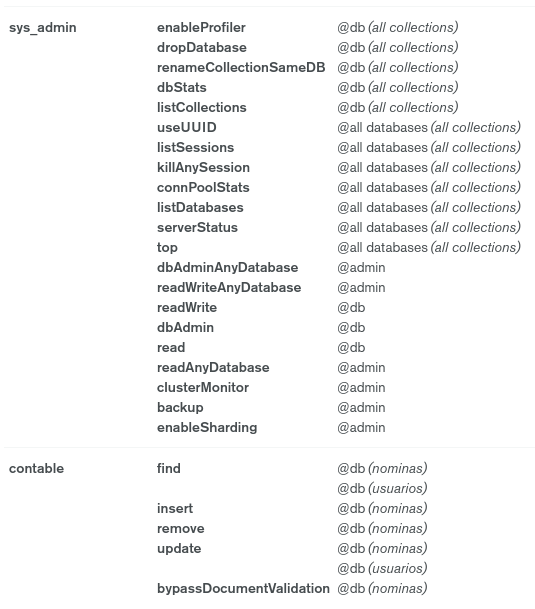
\includegraphics[scale=0.5]{roles.png}\\
  \caption{Roles de administrador de sistemas y de contable}
  \label{fig:select}
\end{figure}

\pagebreak

Algunas de las medidas de seguridad especificadas anteriormente se pueden incorporar, por ejemplo la de acceder a la base de datos desde equipos o servidores específicos [Fig \ref{fig:network_access}] o acceder con credenciales también es posible mediante el uso de LDAP y también se ofrece el encriptado del cluster securizando así el disco [Fig \ref{fig:advanced_access}].
\begin{figure}[ht]
  \centering
  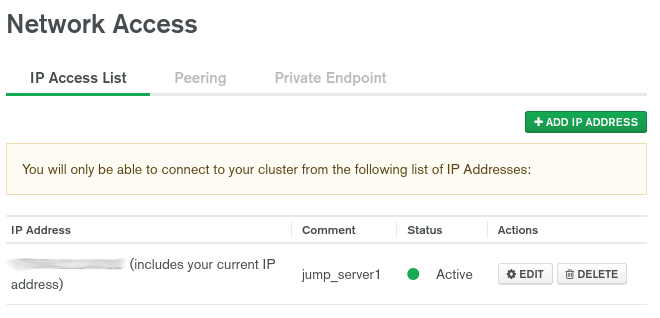
\includegraphics[scale=0.3]{network_access.png}\\
  \caption{Restringir el acceso a unas IPs específicas}
  \label{fig:network_access}

  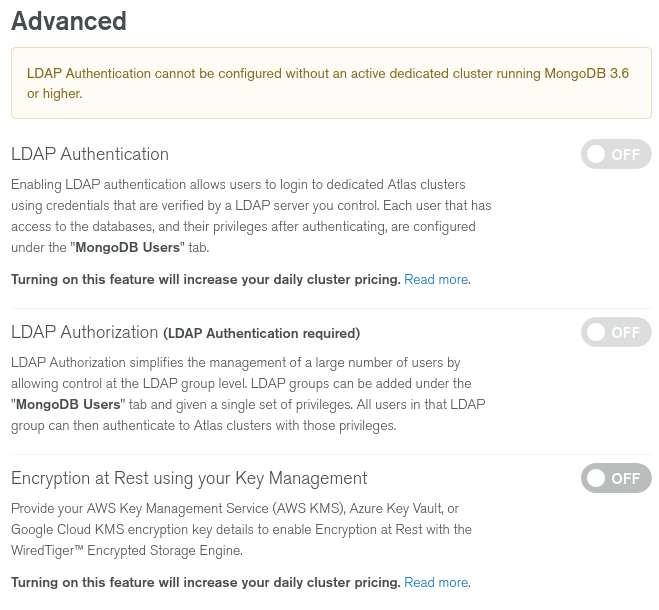
\includegraphics[scale=0.3]{advanced.png}\\
  \caption{Medidas de acceso avanzadas}
  \label{fig:advanced_access}
\end{figure}


\pagebreak
\section{}
Para la realización de este ejercicio y debido a algunas dificultades técnicas se ha utilizado la imagen oficial de Oracle Database 12c para Docker 
\cite{medium} en Ubuntu 20.04 LTS. Docker nos permite deplegar aplicaciones dentro de estructuras virtuales, en este caso, Oracle Database 12c \cite{dockerhub} desde la terminal:
\begin{lstlisting}[language=bash]
docker run -d 
	--name oracle1 
	-p 1521:1521 -p 5500:5500 
	-e ORACLE_SID=DEV 
	-e ORACLE_PDB=TRUNK 
	-e ORACLE_PWD=Databas3 
	-e ORACLE_CHARACTERSET=AL32UTF8 
	store/oracle/database-enterprise:12.2.0.1
\end{lstlisting}

\begin{lstlisting}[language=bash]
docker exec -it oracle1 bash -c "source /home/oracle/.bashrc; sqlplus sys/Oradoc_db1@ORCLCDB as sysdba"
\end{lstlisting}

\subsection{}
Para ver las Bases de Datos que hay creadas por defecto podemos listarlas con la query:

\begin{lstlisting}[language=sql]
SQL> SELECT TABLESPACE_NAME FROM DBA_TABLESPACES;
\end{lstlisting}

\begin{figure}[h!]
  \centering
  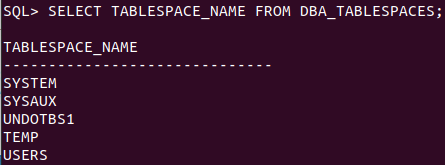
\includegraphics[scale=0.7]{SELECT.png}\\
  \caption{Query para mostrar tablas por defecto}
  \label{fig:select}
\end{figure}

\subsection{}
Un componente importante de una base de datos de Oracle es su diccionario de datos (\textit{data dictionary}), que se trata de un conjunto de tablas de solo lectura que proporciona metadatos de la base de datos. El contenido del diccionario de datos se divide en Base Tables que guardan información sobre la misma base de datos y cuyo acceso lectura/escritura está restringido a la propia base de datos y Views que decodifica las base tables en información inteligible para el usuario \cite{metadata}.\\
De este último conjunto se podrían destacar el siguiente subconjunto de tablas que contienen información relevante.

\begin{itemize}
\item Vistas con prefijo ALL\_: Objetos sobre los que un usuario tiene privilegios
\item Vistas con prefijo USER\_: Objetos que pertencen a un usuario.
\item Vistas con prefijo DBA\_: Contiene todos los objetos con información útil para el administrador. Su uso está restringido al administrador de la base de datos.
\end{itemize}

\subsection{}
Para saber los usuarios que se crean por defecto en la base de datos podemos hacer una consulta sobre la tabla DBA\_USERS que contiene información sobre los usuarios de la base de datos [Fig. \ref{fig:oracle_dba_users}].

\begin{figure}
  \centering
  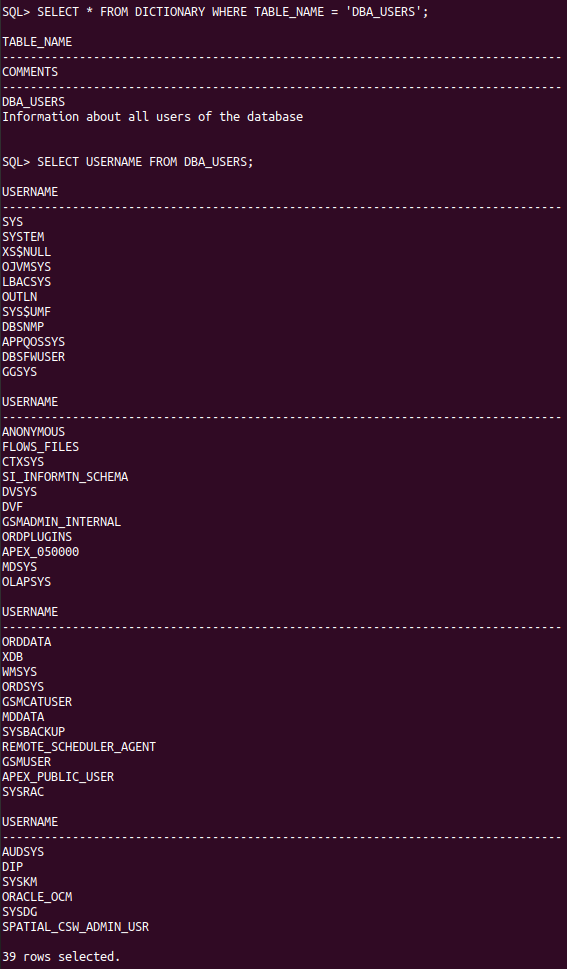
\includegraphics[scale=0.6]{DBAUSERS.png}\\
  \caption{Query para mostrar información de DBA\_USERS y query para mostrar los usuarios de DBA\_USERS}
  \label{fig:oracle_dba_users}
\end{figure}

Para inspeccionar los roles de los usuarios, podemos consultar la tabla DBA\_SYS\_PRIVS y hacer una JOIN con la tabla DBA\_USERS de la siguiente manera:
\begin{lstlisting}[language=sql]
SELECT USERNAME, PRIVILEGE FROM DBA_USERS INNER JOIN DBA_SYS_PRIVS ON DBA_USERS.USERNAME = DBA_SYS_PRIVS.GRANTEE ORDER BY DBA_USERS.USERNAME;
\end{lstlisting}
Sin embargo, esta query genera un resultado de 472 filas, así que se mostrarán los permisos del usuario SYSTEM que tan solo goza de 8 privilegios [Fig. \ref{fig:oracle_priv}].

\begin{figure}[h!]
  \centering
  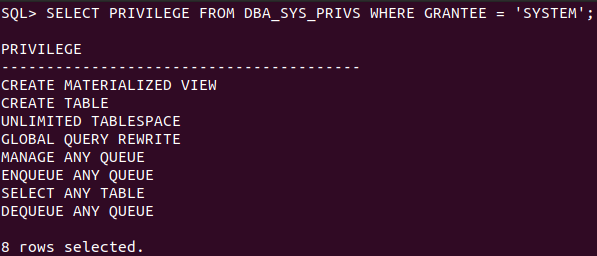
\includegraphics[scale=0.7]{PRIV.png}\\
  \caption{Query para mostrar los permisos del usuario SYSTEM}
  \label{fig:oracle_priv}
\end{figure} 

\pagebreak
\subsection{}
Los puertos a la escucha son el 1521 (Oracle TNS Listener) que pasa las peticiones de un usuario a la instancia de la base de datos a través de la red y el 5500 (OEM Database Express) es una herramienta web incluida en Oracle Database 12c que sirve para administrar distintas areas de la BD (Configuración, Almacenamiento, Seguridad y Rendimiento) \cite{1521} \cite{5500}.

\begin{figure}[h!]
  \centering
  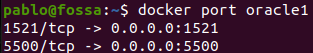
\includegraphics[scale=0.7]{ports.png}\\
  \caption{Listado de puertos activos del container de Oracle Database}
  \label{fig:oracle_ports}
\end{figure} 

Para deshabilitarlos se puede usar el comando ``lsnrctl''\cite{listenerctl}:
\begin{lstlisting}[language=bash]
lsnrctl STOP [listener_name]
\end{lstlisting}

\subsection{}
Los binarios, dentro de la imagen de Docker, se encuentran en el directorio \\
/u01/app/oracle/product/12.2.0/dbhome\_1/bin. [Fig. \ref{fig:oracle_bin}].
\begin{figure}[h!]
  \centering
  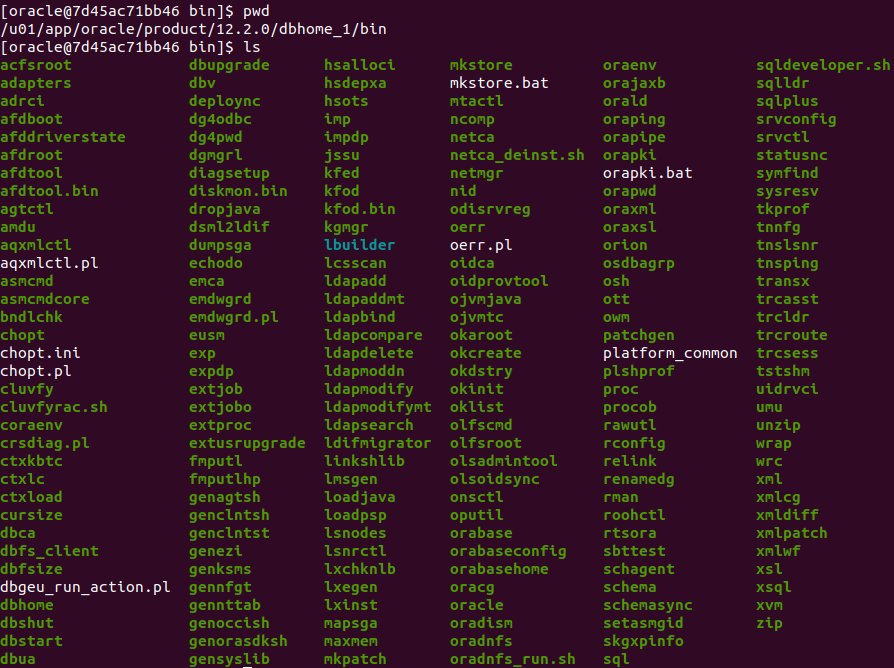
\includegraphics[scale=0.4]{bin.png}\\
  \caption{Archivos binarios de Oracle Database.}
  \label{fig:oracle_bin}
\end{figure}

Los archivos de datos, en cambio, se encuentran en /ORCL/u02/app/oracle/oradata/ORCLCDB \cite{datafiles} [Fig. \ref{fig:oracle_data}].
\begin{figure}[h!]
  \centering
  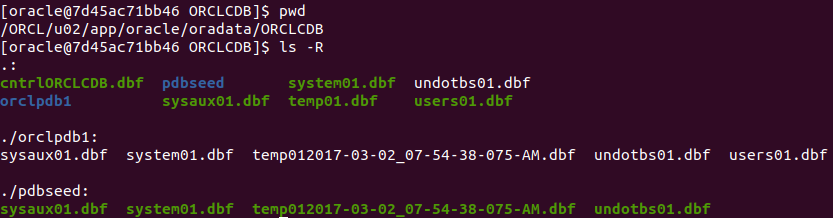
\includegraphics[scale=0.4]{data.png}\\
  \caption{Archivos de datos de Oracle Database.}
  \label{fig:oracle_data}
\end{figure}

\pagebreak
\subsection{}
Los procesos relacionados con Oracle Database en el container se ejecuta con el usuario ``oracle'' con un PID muy elevado [Fig. \ref{fig:oracle_perm}].
\begin{figure}[h!]
  \centering
  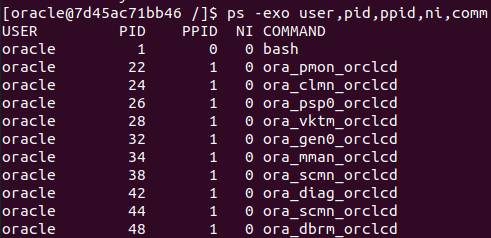
\includegraphics[scale=0.5]{oracle_perm.png}\\
  \caption{Procesos de Oracle en el container}
  \label{fig:oracle_perm}
\end{figure}

\pagebreak
\subsection{}

Durante el proceso de instalación mediante el instalador, en el primer paso llamado ``Configure Security Updates'', nos permite introducir una dirección de correo electrónico en el que recibir notificaciones de seguridad. Más adelante, en el paso llamado ``Typical Installation'', nos permite especificar la contraseña que usarán los usuarios SYS, SYSTEM, SYSMAN y DBSNMP \cite{install_oracle}.

\subsection{}
La instalación de MongoDB Community Server se ha hecho a través del gestor de paquetes dpkg sobre el paquete mongodb-org-server\_4.4.1\_amd64.deb y no ha habido ninguna opción de seguridad disponible. Sin embargo, existe un archivo de configuración para mongo, /etc/mongo.conf, con un apartado de seguridad [Fig. \ref{fig:mongoconf}]. 
\begin{figure}[h!]
  \centering
  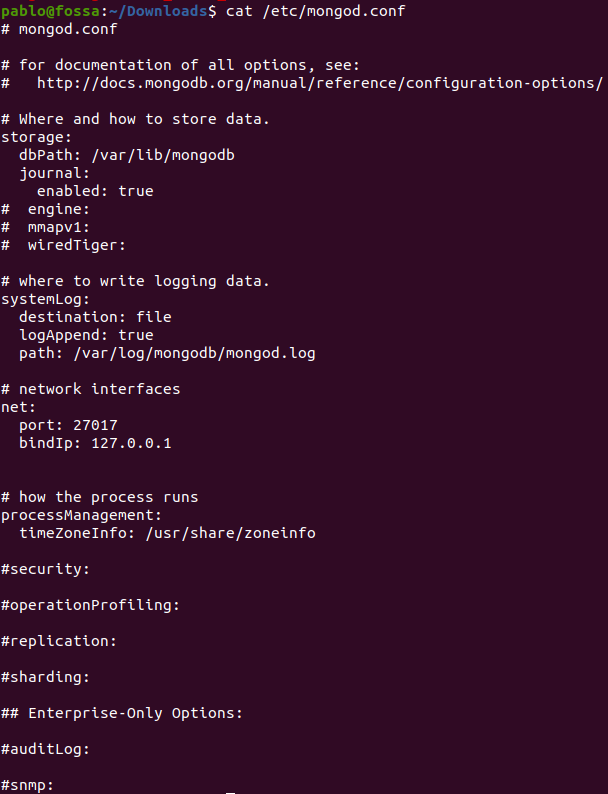
\includegraphics[scale=0.4]{mongoconf.png}\\
  \caption{Archivos de configuración de MongoDB.}
  \label{fig:mongoconf}
\end{figure}

\pagebreak

Por defecto, la seguridad no está aplicada pero en Mongo existen distintas configuraciones para este parámetro [Fig. \ref{fig:mongo_sec}]
\begin{figure}[h!]
  \centering
  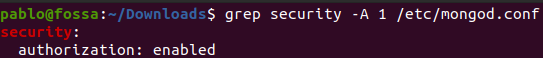
\includegraphics[scale=0.4]{mongosec.png}\\
  \caption{Sección de seguridad en /etc/mongo.conf}
  \label{fig:mongo_sec}
\end{figure}

Con esta configuración se activa el RBAC y de manera implícita la autenticación \cite{mongosec}.

\subsection{}
El puerto por defecto para instancia de mongo y el mongo daemon es el 27017. Existen otros puertos relacionados con la configuración de mongo en modo cluster los 27018 y el 27019 \cite{mongoports}.
Para usar otro puerto se puede editar el archivo /etc/mongo.conf en el apartado de ``net'' [Fig. \ref{fig:mongo_net}].
\begin{figure}[h!]
  \centering
  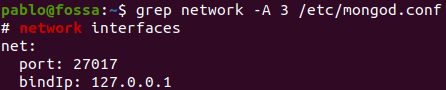
\includegraphics[scale=0.4]{mongonet.png}\\
  \caption{Sección de network en /etc/mongo.conf}
  \label{fig:mongo_net}
\end{figure}

\pagebreak

\subsection{}
El proceso de mongod ha sido ejecutado por el usuario mongodb y con un PID igual a 1.
\begin{figure}[h!]
  \centering
  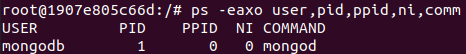
\includegraphics[scale=0.4]{mongod_perm.png}\\
  \caption{Procesos de Mongo en el container}
  \label{fig:mongo_proc}
\end{figure}

\subsection{}
Tanto los binarios como los archivos de datos se encuentran en /data/db donde pondemos encontrar el Storage Engine de WiredTiger, los índices y colecciones de la base de datos y el journaling que mantiene un registro de las operaciones del storage engine \cite{journaling}

\begin{figure}[h!]
  \centering
  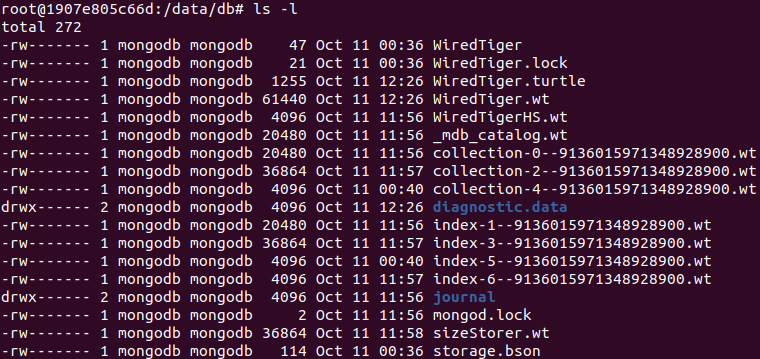
\includegraphics[scale=0.4]{mongobinaries.png}\\
  \caption{Listado de archivos binarios en el sistema}
  \label{fig:mongo_bin}
\end{figure}

\pagebreak
\subsection{}

\begin{tabularx}{\textwidth}{|X|X|X|X|}

\hline
\textbf{Base de Datos} & \textbf{Principales características} & \textbf{Consideración de uso} & \textbf{Aspectos de seguridad relevantes} \\ \hline
\textbf{Oracle} & Software multiplataforma propietario de Oracle. Es una base de datos multimodelo, implementada en C , C++ y ensamblador. Se utiliza para el procesamiento de transacciones en línea y datawarehouse. & Es un producto muy asentado en la industria, con soporte para muchas plataformas y viene avalado por Oracle. Se integra bien con otros servicios de Oracle & Oracle Database tiene una amplia sección de vulnerabilidades. Algunas vulnerabilidades destacables son en un componente del core de Oracle Database Server que da al atacante altos privilegios mediante Oracle Net \cite{oraclesec}\\ \hline

\textbf{MongoDB} & Base de datos documental NoSQL de código abierto, multiplataforma e implementada en C++. Permite indexación de cualquier campo de un documento, replicación y fragmentación & Sistemas con un alto volumen de lecturas. Tiempo real. Manejo de documentos y de contenido & Viene sin configuración de seguridad por defecto. Hay que seleccionar de manera explícita el acceso mediante autorización y el uso de TLS/SSL para todas las conexiones \\ \hline

\textbf{HP Vertica} & Base de datos orientada a columnas diseñada para el manejo de grandes volúmenes de datos con un rendimiento de consulta elevado para datawarehouses. Permite procesamiento paralelo masivo, distintas técnicas machine learning integradas y múltiples interfaces. & Machine learning. Bajo coste. Orientada al cloud computing ya que es independiente de la plataforma y accesible en Amazon Web Service & Existen algunas vulnerabilidades importantes en algunas versiones de HP Vertica que permiten a un usuario remoto obtener privilegios \cite{hpvertsec}\\ \hline

\textbf{Neo4j} & Base de datos multiplataforma orientada a grafos compatible con ACID. Implementada en Java y con licencia dual. Implementa su propio lenguaje de consultas llamado Cypher. & Es una opción a considerar si se desea utilizar una estructura de datos que utilice estructuras de grafos para queries semánticas con nodos, aristas y propiedades o etiquetas para guardar datos con la integridad que proporcionan las bases de datos ACID. &
Existen varias vulnerabilidades de Cross-Site Request Forgery en algunas versiones de Neo4J que permite a un atacante remoto secuestrar la autenticación de administración para ejecutar código arbitrario \cite{neo4jsec}\\ \hline

\textbf{Elastic Search} & Es un motor de búsqueda NoSQL distribuido para hacer búsquedas casi en tiempo real en todo tipo de documentos. Multiplataforma e implementado en Java & Tiene multitud de clientes y está fuertemente acoplado con HTTP y JSON lo cual facilita mucho su interconexión y realizar búsquedas en documentos & Existen varias vulnerabilidades relacionadas con el ELK stack (Elasticsearch, Kibana, Logstash), cabe destacar que en algunas versiones antiguas de Elasticsearch se puede bypasear la protección y ejecutar scripts en remoto \cite{elasticsec} \\ \hline

\textbf{MariaDB} & Base de datos multiplataforma producto derivado de MySQL (base de datos relacional). Utiliza licencia GPL y está implementada en C, C++, Perl y Bash & Tiene más opciones que su predecesor en cuanto a motores de búsqueda. Proprociona estadísticas y otra meta información en nuevas tablas. Más precisión en cuanto a timestamps. Podría considerarse su uso frente a MySQL como una alternativa con más características & En algunas versiones de MariaDB existen vulnerabilidades que permiten a usuarios autenticados bypasear algunas restricciones de acceso y y replicar sentencias DDL en otros nodos \cite{mariadbsec} \\ \hline

\textbf{MS SQL} & Sistema de bases de datos relacional propiedad de Microsoft que a su vez utiliza su propio lenguaje Transact-SQL para funcionar & Puede considerarse frente a otras bases de datos relacionales si se tiene un fuerte acoplamiento o dependencia con otros productos de Microsoft & Una vulnerabilidad muy conocida es muy explotable desde varios frentes, la SQL Server Remote Code Execution Vulnerability \cite{mssqlsec}\\ \hline

\textbf{Redis} & Motor de base de datos en memoria (caché) para el almacenamiento de tablas de tipo diccionario. Soporta 3 tipos de estructuras de datos (Listas, conjuntos y hashes) y antiguamente los datos no eran persistentes puesto que se guardaban en RAM. & Debido al ser un sistema que guarda los datos en RAM puede ser utilizado como base de datos auxiliar antes de utilizar otra con persistencia. Tiene multiplicidad de clientes en varios lenguajes & En algunas versiones existen vulnerabilidades que permiten hacer stack-buffer y head-buffer overflow con el comando SETRANGE \cite{redissec}
\\ \hline

\textbf{PosgreSQL} & Sistema de gestión de base de datos relacional implementado en C de código abierto. La principal característica es su tolerancia a la alta concurrencia lo que permite que varios procesos hagan distintas operaciones sobre una misma tabla sin bloqueos. & Puede considerarse su uso en aplicaciones con alta demanada y concurrencia sin sacrificar la integridad de los datos. & Se han encontrado vulnerabilidades recientes que permiten a un usuario ejecutar código arbitrario en el sistema. Estas vulnerabilidades están relacionadas con el programa ``COPY TO/FROM PROGRAM'' y con stack-buffer overflow \cite{postgresqlsec}
\\ \hline
\caption{Comparación de distintos SGBBDD} 
\label{tab:databasecomp}
\end{tabularx}

\vspace{5cm}

\pagebreak

\begin{thebibliography}{9}

\bibitem{medium}
	\textbf{INSTALAR ORACLE Database 12c CON DOCKER}\\
	\textit{Jeremy Andress}\\
	\url{https://medium.com/@jeremyandress/instalar-oracle-database-12c-con\\-docker-3a18d534c7b0}

\bibitem{dockerhub}
	\textbf{DockerHub}\\
	Oracle Database Server Docker Image Documentation
	\url{https://hub.docker.com/u/pabloriutort/content/sub-25333d4f-432c-4efb-8c05-49a69e19f165}
	
\bibitem{metadata}
  \textbf{Data Dictionary and Dynamic Performance Views}\\
  Oracle Help Center - Database Concepts\\
  \url{https://docs.oracle.com/database/121/CNCPT/datadict.htm#CNCPT1209}
 
\bibitem{1521}
	\textbf{SANS ISC InfoSec Forums}\\
	Cyber Security Awareness Month - Day 16 - Port 1521 - Oracle TNS Listener\\
	\url{https://isc.sans.edu/forums/diary/Cyber+Security+Awareness+Month+Day+16+Port+1521+Oracle+TNS+Listener/7375/}

\bibitem{5500}
	\textbf{DBA Junior}\\
	Setup OEM Database Express\\
	\url{http://www.dbajunior.com/setup-oem-database-express/}

\bibitem{datafiles}
	\textbf{Oracle - Ask Tom}\\
	about directory location of oracle database files,has it haven one parameter?\\
	\url{https://asktom.oracle.com/pls/apex/f?p=100:11:0::::P11_QUESTION_ID:9535318000346869801}

\bibitem{listenerctl}
	\textbf{Database Net Services Reference}\\
	Listener Control Utility\\
	\url{https://docs.oracle.com/cd/B19306_01/network.102/b14213/lsnrctl.htm}

\bibitem{install_oracle}
	\textbf{Oracle - Help Center}\\
	Installing Oracle Database Software and Creating a Database\\
	\url{https://www.oracle.com/webfolder/technetwork/tutorials/obe/db/12c/r2/2day_dba/12cr2db_ch2install/12cr2db_ch2install.html}

\bibitem{mongosec}
	\textbf{MongoDB Documentation}\\
	Security\\
	\url{https://docs.mongodb.com/manual/security/}

\bibitem{mongoports}
	\textbf{MongoDB Documentation}\\
	Default MongoDB Port\\
	\url{https://docs.mongodb.com/manual/reference/default-mongodb-port/}

\bibitem{journaling}
	\textbf{MongoDB Documentation}\\
	Journaling\\
	\url{https://docs.mongodb.com/manual/core/journaling/}

\bibitem{oraclesec}
	\textbf{CVE Details}\\
	Oracle Database Security Vulnerabilities\\
	\url{https://www.cvedetails.com/vulnerability-list/vendor_id-93/product_id-18751/version_id-221169/Oracle-Database-12.2.0.1.html}

\bibitem{hpvertsec}
	\textbf{CVE Details}\\
	HP Vertica Security Vulnerabilities\\
	\url{https://www.cvedetails.com/vulnerability-list/vendor_id-10/product_id-32574/HP-Vertica.html}

\bibitem{neo4jsec}
	\textbf{CVE Details}\\
	Neo4J Security Vulnerabilities [CVE-2013-7259]\\
	\url{https://www.cvedetails.com/cve/CVE-2013-7259/}

\bibitem{elasticsec}
	\textbf{CVE Details}\\
	Elasticsearch Security Vulnerabilities\\
	\url{https://www.cvedetails.com/vulnerability-list/vendor_id-13554/Elasticsearch.html}

\bibitem{mariadbsec}
	\textbf{CVE Details}\\
	MariaDB 10.2.0 Security Vulnerabilities\\
	\url{https://www.cvedetails.com/vulnerability-list/vendor_id-12010/product_id-22503/version_id-207752/Mariadb-Mariadb-10.2.0.html}

\bibitem{mssqlsec}
	\textbf{CVE Details}\\
	Miscroft SQL Server Vulnerabilities\\
	\url{https://www.cvedetails.com/vulnerability-list/vendor_id-26/product_id-251/Microsoft-Sql-Server.html}

\bibitem{redissec}
	\textbf{CVE Details}\\
	Redis Vulnerabilities\\
	\url{https://www.cvedetails.com/vulnerability-list/vendor_id-18560/product_id-47087/version_id-307209/Redislabs-Redis-5.0.3.html}

\bibitem{postgresqlsec}
	\textbf{CVE Details}\\
	Postgresql Vulnerabilities\\
	\url{https://www.cvedetails.com/vulnerability-list/vendor_id-336/product_id-575/year-2019/opec-1/Postgresql-Postgresql.html}

\end{thebibliography}

\end{document}